\documentclass[]{beamer}
%\documentclass[handout]{beamer}
% ***************************************************************
% for handout, change only this...
%   \documentclass[twocolumn]{article}
%   \usepackage{beamerarticle}
%   \setlength{\textwidth}{7.5in}
%   \setlength{\textheight}{9.8in}
%   \setlength{\topmargin}{-1in}
%   \setlength{\oddsidemargin}{-.52in}
%   \setlength{\evensidemargin}{-.52in}

%\usepackage{beamerprosper}
%\usetheme{Warsaw}
%\usecolortheme{orchid}

\usepackage{graphicx}
\usepackage{amsmath,amssymb,array,comment,eucal}
\usepackage{xcolor}
\definecolor{beamer@blendedblue}{RGB}{86,155,189}
\definecolor{myblue}{RGB}{12,76,138}
\setbeamercolor{structure}{fg=myblue}
\definecolor{Ftitle}{RGB}{12,76,138}
\definecolor{Descitem}{RGB}{238,238,244}
\definecolor{StdTitle}{RGB}{12,76,138}
\definecolor{StdBody}{RGB}{213,24,0}
\definecolor{StdBody}{RGB}{213,24,0}

\definecolor{AlTitle}{RGB}{255, 190, 190}
\definecolor{AlBody}{RGB}{213,24,0}

\definecolor{ExTitle}{RGB}{201, 217, 217}
\definecolor{ExBody}{RGB}{213,24,0}

\setbeamercolor{frametitle}{fg = Ftitle}
\setbeamercolor{title}{fg = Ftitle}
\setbeamercolor{item}{fg = Ftitle}
\setbeamercolor{subitem}{fg = Ftitle}
\setbeamercolor{subsubitem}{fg = Ftitle}
\setbeamercolor{description item}{fg = myblue}
\setbeamercolor{titlelike}{fg=myblue}

\DeclareMathOperator{\sgn}{sgn}
\newcommand{\e}{\mathbf{e}}
\renewcommand{\P}{\mathbf{P}}
\newcommand{\F}{\mathbf{F}}
\newcommand{\R}{\textsf{R}}
\newcommand{\mat}[1] {\mathbf{#1}}
%\newcommand{\ind}{\mathrel{\mathop{\sim}\limits^{\mathit{ind}}}}
%\newcommand{\iid}{\mathrel{\mathop{\sim}\limits^{\mathit{iid}}}}
\newcommand{\E}{\textsf{E}}
\newcommand{\SE}{\textsf{SE}}
\newcommand{\SSE}{\textsf{SSE}}
\newcommand{\RSS}{\textsf{RSS}}
\newcommand{\FSS}{\textsf{FSS}}
\renewcommand{\SS}{\textsf{SS}}
\newcommand{\MSE}{\textsf{MSE}}
\newcommand{\SSR}{\textsf{SSR}}
\newcommand{\Be}{\textsf{Beta}}
\newcommand{\St}{\textsf{St}}
\newcommand{\Ca}{\textsf{C}}
\newcommand{\Exp}{\textsf{Exp}}
\newcommand{\GDP}{\textsf{GDP}}
\newcommand{\NcSt}{\textsf{NcSt}}
\newcommand{\Bin}{\textsf{Bin}}
\newcommand{\NB}{\textsf{NegBin}}
\renewcommand{\NG}{\textsf{NG}}
\newcommand{\N}{\textsf{N}}
\newcommand{\Ber}{\textsf{Ber}}
\newcommand{\Poi}{\text{Poi}}
\newcommand{\Gam}{\textsf{Gamma}}
\newcommand{\BB}{\textsf{BB}}
\newcommand{\Gm}{\textsf{G}}
\newcommand{\Un}{\textsf{Unif}}
\newcommand{\Ex}{\textsf{Exp}}
\newcommand{\DE}{\textsf{DE}}
\newcommand{\tr}{\textsf{tr}}
\newcommand{\cF}{{\cal{F}}}
\newcommand{\cL}{{\cal{L}}}
\newcommand{\cI}{{\cal{I}}}
\newcommand{\cB}{{\cal{B}}}
\newcommand{\cP}{{\cal{P}}}
\newcommand{\bbR}{\mathbb{R}}
\newcommand{\bbN}{\mathbb{N}}
\newcommand{\pperp}{\mathrel{{\rlap{$\,\perp$}\perp\,\,}}}
\newcommand{\OFP}{(\Omega,\cF, \P)}
\newcommand{\eps}{\boldsymbol{\epsilon}}
\newcommand{\1}{\mathbf{1}_n}
\newcommand{\gap}{\vspace{8mm}}
\newcommand{\ind}{\mathrel{\mathop{\sim}\limits^{\rm ind}}}
\newcommand{\simiid}{\ensuremath{\mathrel{\mathop{\sim}\limits^{\rm
iid}}}}
\newcommand{\eqindis}{\ensuremath{\mathrel{\mathop{=}\limits^{\rm D}}}}
\newcommand{\iid}{\textit{i.i.d.}}
\newcommand{\SSZ}{S_{zz}}
\newcommand{\SZW}{S_{zw}}
\newcommand{\Var}{\textsf{Var}}
\newcommand{\corr}{\textsf{corr}}
\newcommand{\diag}{\textsf{diag}}
\newcommand{\var}{\textsf{var}}
\newcommand{\Cov}{\textsf{Cov}}
\newcommand{\Sam}{{\cal S}}
\def\H{\mathbf{H}}
\newcommand{\I}{\mathbf{I}}
\newcommand{\Y}{\mathbf{Y}}
\newcommand{\tY}{\tilde{\mathbf{Y}}}
\newcommand{\Yhat}{\hat{\mathbf{Y}}}
\newcommand{\Yobs}{\mathbf{Y}_{{\cal S}}}
\newcommand{\barYobs}{\bar{Y}_{{\cal S}}}
\newcommand{\barYmiss}{\bar{Y}_{{\cal S}^c}}
\def\bv{\mathbf{b}}
\def\X{\mathbf{X}}
\def\tX{\tilde{\mathbf{X}}}
\def\x{\mathbf{x}}
\def\xbar{\bar{\mathbf{x}}}
\def\Xbar{\bar{\mathbf{X}}}
\def\Xg{\mathbf{X}_{\boldsymbol{\gamma}}}
\def\Ybar{\bar{\Y}}
\def\ybar{\bar{y}}
\def\y{\mathbf{y}}
\def\Yf{\mathbf{Y_f}}
\def\W{\mathbf{W}}
\def\L{\mathbf{L}}
\def\w{\mathbf{w}}
\def\U{\mathbf{U}}
\def\V{\mathbf{V}}
\def\Q{\mathbf{Q}}
\def\Z{\mathbf{Z}}
\def\z{\mathbf{z}}
\def\v{\mathbf{v}}
\def\u{\mathbf{u}}

\def\zero{\mathbf{0}}
\newcommand{\one}{\mathbf{1}}
\newcommand{\taub}{\boldsymbol{\tau}}
\newcommand{\betav}{\boldsymbol{\beta}}
\newcommand{\alphav}{\boldsymbol{\alpha}}
\newcommand{\A}{\mathbf{A}}
\def\a{\mathbf{a}}
\def\K{\mathbf{K}}
\newcommand{\B}{\mathbf{B}}
\def\b{\boldsymbol{\beta}}
\def\bhat{\hat{\boldsymbol{\beta}}}
\def\btilde{\tilde{\boldsymbol{\beta}}}
\def\tb{\boldsymbol{\theta}}
\def\bg{\boldsymbol{\beta_\gamma}}
\def\bgnot{\boldsymbol{\beta_{(-\gamma)}}}
\def\mub{\boldsymbol{\mu}}
\def\tmub{\tilde{\boldsymbol{\mu}}}
\def\muhat{\hat{\boldsymbol{\mu}}}
\def\tb{\boldsymbol{\theta}}
\def\tk{\boldsymbol{\theta}_k}
\def\tj{\boldsymbol{\theta}_j}
\def\Mk{\boldsymbol{{\cal M}}_k}
\def\M{\boldsymbol{{\cal M}}}
\def\Mj{\boldsymbol{{\cal M}}_j}
\def\Mi{\boldsymbol{{\cal M}}_i}
\def\Mg{{\boldsymbol{{\cal M}_\gamma}}}
\def\Mnull{\boldsymbol{{\cal M}}_{N}}
\def\gMPM{\boldsymbol{\gamma}_{\text{MPM}}}
\def\gHPM{\boldsymbol{\gamma}_{\text{HPM}}}
\def\Mfull{\boldsymbol{{\cal M}}_{F}}
\def\tg{\boldsymbol{\theta}_{\boldsymbol{\gamma}}}
\def\g{\boldsymbol{\gamma}}
\def\eg{\boldsymbol{\eta}_{\boldsymbol{\gamma}}}
\def\G{\mathbf{G}}
\def\cM{\cal M}
\def\D{\Delta}
\def \shat{{\hat{\sigma}}^2}
\def\uv{\mathbf{u}}
\def\l {\lambda}
\def\d{\delta}
\def\Sigmab{\boldsymbol{\Sigma}}
\def\Lambdab{\boldsymbol{\Lambda}}
\def\lambdab{\boldsymbol{\lambda}}
\def\Mg{{\cal M}_\gamma}
\def\S{{\cal{S}}}
\def\qg{p_{\boldsymbol{\gamma}}}
\def\pg{p_{\boldsymbol{\gamma}}}
%\def\t{\mathbf{t}}
\def\T{\boldsymbol{\Theta}}
\def\Tb{\boldsymbol{\Theta}}

\title{Bayesian Model Choice}

\author{Hoff Chapter 9, Liang et al 2007, Hoeting et al (1999), Clyde \&
 George (2004) Statistical Science}
\date{\today}
%\Logo(-1.9,7.3){
\includegraphics[width=.5in]{../eps/duke}}
% Optional: text to put in the bottom of each slide.
% By default, the title of the talk will be placed there.
%\slideCaption{\textit{October 28, 2005 }}

\usepackage{Sweave}
\begin{document}
\Sconcordance{concordance:15-model-choice.tex:15-model-choice.Rnw:%
1 29 1 1 0 4 1 1 6 510 1}

% make the title slide
\maketitle


\begin{frame}
  \frametitle{Posterior Distribution}
With a Normal-Gamma Prior $\NG(\bv_0, \Phi_0, \nu_0, \SS_0)$, the posterior is $\NG(\bv_n, \Phi_n, \nu_n, \SS_n))$: with 

\begin{eqnarray*}
\b \mid \phi, \Y & \sim &\N(\bv_n, (\phi \Phi_n)^{-1}) \pause \\
\phi \mid \Y &\sim &\G(\frac{\nu_n}{2}, \frac{\SS_n}{2})
  \end{eqnarray*}

and hyper-parameters
  \begin{eqnarray*}
\Phi_n & = & \X^T\X +  \Phi_0 \pause \\
\bv_n  & = & \Phi_n^{-1} (\X^T\X \bhat  + \Phi_0 \bv_0) \pause \\
\nu_n & = &  n + \nu_0 \pause \\
\SS_n & = &\SSE + \SS_0 + \bhat^T \X^T\X \bhat + \bv_0^T \Phi_0 \bv_0
 - \bv_n^T \Phi_n \bv_n
  \end{eqnarray*}


\end{frame}
\begin{frame}
  \frametitle{Marginal Distribution from Normal--Gamma }
  \begin{theorem}
    Let  $\tb \mid \phi \sim \N(m, \frac{1}{\phi} \Sigma)$ and $\phi \sim
    \G(\nu/2, \nu \shat/2)$. Then  $\tb$ ($p \times 1)$ has a $p$
    dimensional multivariate $t$ distribution $$\tb \sim t_\nu( m,
    \shat \Sigma )$$ with density
$$p(\tb) \propto  \left[ 1 + \frac{1}{\nu}  \frac{ (\tb - m)^T
    \Sigma^{-1} (\tb - m)}{\shat} \right]^{- \frac{p + \nu}{2}}$$
  \end{theorem}
\end{frame}

\begin{frame}
  \frametitle{Derivation}
Marginal density  $p(\tb) = \int p(\tb \mid \phi) p(\phi) \, d\phi$
\pause
\begin{eqnarray*}
  p(\tb) & \propto & \int |\Sigma/\phi|^{-1/2}
e^{- \frac{\phi}{2} (\tb - m)^T
    \Sigma^{-1} (\tb - m)}  \phi^{\nu/2 - 1} e^{- \phi \frac{\nu
      \shat}{2}}\, d \phi \pause \\
  & \propto & \int \phi^{p/2} \phi^{\nu/2 - 1}
e^{- \phi \frac{(\tb - m)^T
    \Sigma^{-1} (\tb - m)+  \nu
      \shat}{2}}\, d \phi \pause \\
 & \propto & \int \phi^{\frac{p +\nu}{2} - 1}
e^{- \phi \frac{(\tb - m)^T
    \Sigma^{-1} (\tb - m)+  \nu
      \shat}{2}} \, d \phi \pause \\
& = & \Gamma((p + \nu)/2 ) \left( \frac{(\tb - m)^T
    \Sigma^{-1} (\tb - m)+  \nu
      \shat}{2} \right)^{- \frac{p + \nu}{2}} \pause \\
& \propto &  \left( (\tb - m)^T
    \Sigma^{-1} (\tb - m)+  \nu
      \shat \right)^{- \frac{p + \nu}{2}} \pause \\
& \propto &  \left( 1 + \frac{1}{\nu}  \frac{(\tb - m)^T
    \Sigma^{-1} (\tb - m)}{\shat}
       \right)^{- \frac{p + \nu}{2}}
\end{eqnarray*}
\end{frame}

\begin{frame}
  \frametitle{Marginal Posterior Distribution of $\b$}
  \begin{eqnarray*}
\b \mid \phi, \Y  & \sim & \N( \bv_n, \phi^{-1} \Phi_n^{-1}) \pause \\
 \phi \mid \Y & \sim & \G\left(\frac{\nu_n}{2},  \frac{\SS_n}{ 2} \right)
  \end{eqnarray*}
\pause

Let $\shat = \SS_n/\nu_n$  (Bayesian MSE) \pause

Then the marginal posterior distribution of $\b$ is
$$
\b  \mid \Y \sim t_{\nu_n} (\bv_n, \shat \Phi_n^{-1})
$$ \pause


Any linear combination $\x^T\b$
$$\x^T\b  \mid \Y \sim t_{\nu_n}
(\x^T\bv_n, \shat \x^T\Phi_n^{-1}\x)$$ has a univariate
$t$ distribution with $\v_n$ degrees of freedom

\end{frame}

\begin{frame}
  \frametitle{Predictive Distribution}
Suppose $\Y^* \mid \b, \phi \sim \N(\X^* \b , \I/\phi)$  and is conditionally
independent of $\Y$ given $\b$ and $\phi$ \pause
\vspace{18pt}

What is the predictive distribution of $\Y^* \mid \Y$? \pause

\vspace{18pt}
$\Y^* = \X^* \b + \eps^*$ and $\eps^*$ is independent of $\Y$ given
$\phi$ \pause

\begin{eqnarray*}
\X^* \b + \eps^* \mid \phi, \Y & \sim & \N(\X^*\bv_n, (\X^{*} \Phi_n^{-1} \X^{*T}
+ \I)/\phi)  \pause \\
\Y^* \mid \phi, \Y & \sim & \N(\X^*\bv_n, (\X^{*} \Phi_n^{-1} \X^{*T}
+ \I)/\phi)  \pause \\
\phi \mid \Y & \sim & \G\left(\frac{\nu_n}{2},
  \frac{\shat \nu_n}{ 2} \right)  \pause \\
\Y^* \mid \Y & \sim & t_{\nu_n}( \X^*\bv_n, \shat (\I + \X^* \Phi_n^{-1} \X^T))
\end{eqnarray*}
\end{frame}
\begin{frame}
  \frametitle{Alternative Derivation}
Conditional Distribution:
\begin{eqnarray*}
f(\Y^* \mid \Y) & = & \frac{f(\Y^*, \Y)}{f(\Y)} \pause \\
 & = & \frac{
\iint f(\Y^*, \Y \mid \b, \phi) p(\b, \phi) d\b\, d\phi
}
{
  f(\Y)
}  \pause \\
 & = & \frac{
\iint f(\Y^*\mid \b, \phi) f(\Y \mid \b, \phi) p(\b, \phi) d\b\, d\phi
}
{
  f(\Y)
}  \pause \\
 & = &
\iint f(\Y^*\mid \b, \phi)  p(\b, \phi \mid \Y) d\b\, d\phi \pause
\end{eqnarray*}

Requires completing the square/quadratic!

\end{frame}

\begin{frame}
  \frametitle{Conjugate Priors}
  \begin{definition}
    A class of prior distributions $\cP$ for $\tb$ is conjugate for a
    sampling model $p(y \mid \tb)$ if for every $p(\tb) \in \cP$, $p(\tb
    \mid \Y) \in \cP$.
  \end{definition}
\pause
  Advantages: \pause
  \begin{itemize}
  \item Closed form distributions for most quantities; bypass MCMC for
    calculations \pause
  \item Simple updating in terms of sufficient statistics ``weighted
    average'' \pause
  \item Interpretation as prior samples - prior sample size \pause
  \item Elicitation of prior through imaginary or historical data \pause
  \item limiting ``non-proper'' form recovers MLEs \pause
  \end{itemize}
Choice of conjugate prior?
\end{frame}

\begin{frame}
  \frametitle{Jeffreys Prior}

Jeffreys proposed a default  procedure so that resulting prior
would be invariant to model parameterization  \pause

$$p(\tb) \propto |\cI(\tb)|^{1/2}$$
\pause
where $\cI(\tb)$ is the  Expected Fisher Information matrix
\pause
$$
\cI(\theta) = - \E[ \left[ \frac{\partial^2 \log(\cL(\tb))}{\partial
  \theta_i \partial \theta_j} \right] ]
$$
\end{frame}
\begin{frame}
  \frametitle{Fisher Information Matrix}
Log Likelihood
$$
    \log(\cL(\b, \phi))  =  \, \frac{n}{2} \log(\phi)  - \frac{\phi}{2}
     \| (\I - \P_\x) \Y\|^2
 - \frac{\phi}{2}(\b - \bhat)^T(\X^T\X)(\b - \bhat)
$$ \pause
  \begin{eqnarray*}
\frac{\partial^2 \log \cL} { \partial \tb \partial \tb^T} & = &
\left[
  \begin{array}{cc}
    -\phi (\X^T\X) & -(\X^T\X) (\b - \bhat) \\
  - (\b - \bhat)^T (\X^T\X) & -\frac{n}{2} \frac{1}{\phi^2} \\
  \end{array}
\right] \pause \\
\E[\frac{\partial^2 \log \cL} { \partial \tb \partial \tb^T}] & = &
\left[
  \begin{array}{cc}
    -\phi (\X^T\X) & \zero_p \\
  \zero_p^T & -\frac{n}{2} \frac{1}{\phi^2} \\
  \end{array}
\right] \pause \\
& & \\
\cI((\b, \phi)^T) & = & \left[
  \begin{array}{cc}
    \phi (\X^T\X) & \zero_p \\
  \zero_p^T & \frac{n}{2} \frac{1}{\phi^2}
  \end{array}
\right]
  \end{eqnarray*}
\end{frame}
\begin{frame}
  \frametitle{Jeffreys Prior}
  Jeffreys Prior
  \begin{eqnarray*}
  p_J(\b, \phi)  & \propto & |\cI((\b, \phi)^T) |^{1/2}   \pause \\
               & = & |\phi (\X^T\X|^{1/2} \left(\frac{n}{2}
                 \frac{1}{\phi^2} \right)^{1/2} \pause \\
  & \propto  &  \phi^{p/2 - 1} |\X^T\X|^{1/2} \pause \\
  & \propto & \phi^{p/2 - 1}  \pause
  \end{eqnarray*}
  Improper prior   $\iint p_J(\b, \phi) \, d\b \, d\phi $ not finite

\end{frame}
\begin{frame}
  \frametitle{Formal Bayes Posterior}
$$  p(\b, \phi \mid \Y) \propto p(\Y \mid \b, \phi)  \phi^{p/2 - 1} $$
\pause
if this is integrable, then renormalize to obtain formal posterior
distribution \pause


\begin{eqnarray*}
  \b \mid \phi, \Y & \sim & \N(\bhat, (\X^T\X)^{-1} \phi^{-1}) \\
  \phi \mid \Y & \sim& \G(n/2, \| \Y - \X\bhat \|^2/2)
\end{eqnarray*} \pause
Limiting case of Conjugate prior with $\bv_0 = 0$, $\Phi = \zero$,
$\nu_0 = 0$ and $\SS_0 = 0$ \pause

  \pause

\vfill
Jeffreys did not recommend using this Posterior does not depend on dimension $p$
\end{frame}
\begin{frame}
  \frametitle{Independent Jeffreys Prior}
  \begin{itemize}
  \item  Treat $\b$ and $\phi$ separately  (``orthogonal
    parameterization'') \pause
  \item $p_{IJ}(\b) \propto |\cI(\b)|^{1/2}$ \pause
\item $p_{IJ}(\phi) \propto |\cI(\phi)\|^{1/2}$ \pause
  \end{itemize}
$$
\cI((\b, \phi)^T)  =  \left[
  \begin{array}{cc}
    \phi (\X^T\X) & \zero_p \\
  \zero_p^T & \frac{n}{2} \frac{1}{\phi^2}
  \end{array}
\right]
$$
\pause
$$p_{IJ}(\b) \propto |\phi \X^T\X|^{1/2} \propto 1$$ \pause
$$p_{IJ}(\phi) \propto \phi^{-1}$$ \pause

Independent Jeffreys Prior is
$$p_{IJ}(\beta, \phi) \propto p_{IJ}(\b) p_{IJ}(\phi) = \phi^{-1}$$

\end{frame}
\begin{frame}
  \frametitle{Formal Posterior Distribution}
  With Independent Jeffreys Prior
$$p_{IJ}(\beta, \phi) \propto p_{IJ}(\b) p_{IJ}(\phi) = \phi^{-1}$$
\pause
Formal Posterior Distribution
\pause
\begin{eqnarray*}
  \b \mid \phi, \Y & \sim & \N(\bhat, (\X^T\X)^{-1} \phi^{-1}) \pause \\
  \phi \mid \Y & \sim& \G((n-p)/2, \| \Y - \X\bhat \|^2/2) \pause\\
\b \mid \Y & \sim & t_{n-p}(\bhat, \shat (\X^T\X)^{-1})\pause
\end{eqnarray*}
Bayesian Credible Sets
$p(\b \in C_\alpha) = 1- \alpha$ correspond to frequentist Confidence
Regions

$$\frac{\lambdab^T\b - \lambdab\bhat}
{\sqrt{\shat \lambdab^T(\X^T\X)^{-1} \lambdab}} \sim t_{n-p}$$

\end{frame}

\begin{frame}
  \frametitle{Zellner's $g$-prior}
Zellner's g-prior(s) $\b \mid \phi \sim \N(\bv_0, g
    (\X^T\X)^{-1}/\phi)$ \pause

$$\b \mid \Y, \phi \sim \N\left( \frac{g}{1 + g} \bhat +  \frac{1}{1 + g}
\bv_0, \frac{g}{1 + g} (\X^T\X)^{-1} \phi^{-1} \right)$$ \pause

\begin{itemize}
\item Invariance: Require posterior of   $\X \b$  equal the posterior of $\X \H \alphav$
\pause   ($\a_0 = \H^{-1} \bv_0$)  (  $\bv_0 = \zero$)

\item Choice of $g$?  \pause
\item $\frac{g}{1 + g}$  weight given to the data \pause
\item Fixed $g$ effect does not vanish as $n \to \infty$
\item Use $g = n$ or place a prior diistribution on $g$
\end{itemize}


\end{frame}
\begin{frame}
  \frametitle{Shrinkage}
 Posterior mean under  $g$-prior  with $\bv_0 = 0$
$\frac{g}{1 +g} \bhat $

\centerline{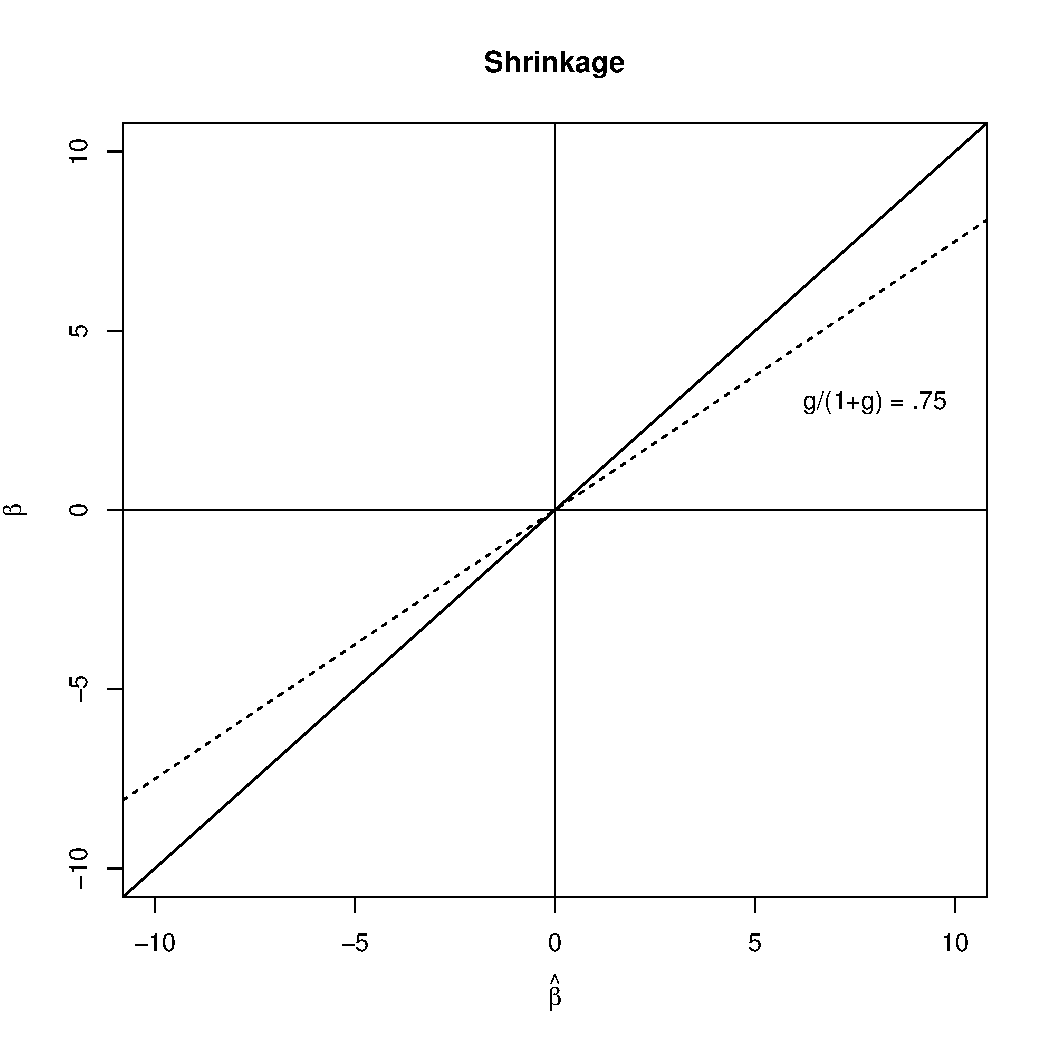
\includegraphics[height=3in]{shrinkage}}
\end{frame}


\begin{frame}\frametitle{Ridge Regression}

\begin{itemize}

\item If $\X^T\X$ is nearly singular, certain  elements of $\b$ or (linear combinations of $\b$) may have huge variances under the $g$-prior (or flat prior) as the MLEs are highly unstable!


\item {\bf Ridge regression} protects against the explosion of variances and ill-conditioning with the conjugate prior:

$$\b \mid \phi \sim \textsf{N}(0, \frac{1}{\phi \lambda} \I_p)$$

\item Posterior for $\b$  (conjugate case)

$$\b \mid \phi, \lambda, \Y \sim \N \left((\lambda \I_p + \X^T\X)^{-1} \X^T \Y,  \frac{1}{\phi}(\lambda \I_p + \X^T\X)^{-1}\right)$$

\item induces shrinkage as well!
\end{itemize}
\end{frame}

\begin{frame} \frametitle{Model Choice ?}
\begin{itemize}
  \item Redundant variables lead to unstable estimates \pause
  \item Some variables may not be relevant ($\beta_j = 0$) \pause
  \item Can we infer a "good" model from the data?
  \item Expand model hierarchically to introduce another latent variable $\g$ that encodes models $\Mg$
  $\g = (\gamma_1, \gamma_2, \ldots \gamma_p)^T$ where
  \begin{align*}
  \gamma_j = 0 & \Leftrightarrow \beta_j = 0 \\
  \gamma_j = 1 &  \Leftrightarrow \beta_j \neq 0 
  \end{align*}
  \item Find Bayes factors and posterior probabilities of models $\Mg$
  \item $2^p$ models!
  
  
  
\end{itemize}


\end{frame}


\begin{frame}\frametitle{Zellner's g-prior}
  Centered model:  $$\Y = \1 \alpha + \X^c \b + \epsilon$$
  where $\X^c$ is the centered design matrix where all variables have
  had their mean subtracted \pause
\begin{itemize}
\item   $p(\alpha, \phi) \propto 1/\phi$ \pause
\item  $\b_\gamma \mid \alpha, \phi, \g \sim \N(0, g \phi^{-1}
  ({\Xg^c}^\prime \Xg^c)^{-1})$ \pause
%\item  take $g=n$
\end{itemize}
which leads to marginal likelihood of $\g$ that is proportional
to $$ p(\Y \mid \g) = C (1 + g)^{\frac{n-p-1}{2}} ( 1 + g (1 -
 R^2_\gamma))^{- \frac{(n-1)}{2}}$$
where $R^2$ is the usual coefficient of determination for model $\Mg$.
\pause

Trade-off of model complexity versus goodness of fit

\bigskip
Lastly, assign distribution to space of models
\end{frame}

\begin{frame}{Sketch}
\begin{itemize}
  \item  Integrate out $\bg$  using sums of normals \pause
  \item  Find inverse of $\I_n + g \P_{\Xg}$  (properties of projections) \pause
  \item Find determinant of $\phi (\I_n + g \P_{\Xg})$  \pause
  \item Integrate out intercept (normal)  \pause
  \item Integrate out $\phi$  (gamma)  \pause
  \item algebra to simplify quadratic forms to  $R^2_{\g}$
\end{itemize}

Or integrate $\alpha$, $\bg$ and $\phi$  (complete the square!)
\end{frame}
\begin{frame}
  \frametitle{Priors on Model Space}
  $p(\Mg) \Leftrightarrow p(\g)$
  \begin{itemize}
  \item $p(\gamma_j = 1) = .5 \Rightarrow P(\Mg) = .5^p$  Uniform on space of models \pause $\pg \sim \Bin(p, .5)$
\item $\gamma_j \mid \pi \simiid \Ber(\pi)$ and $\pi \sim \Be(a,b)$ then  $\pg \sim \BB_p(a, b)$
$$
p(\pg \mid p, a, b) = \frac{ \Gamma(p + 1) \Gamma(\pg + a) \Gamma(p - \pg + b) \Gamma (a + b) }{\Gamma(\pg+1) \Gamma(p - \pg + 1) \Gamma(p + a + b) \Gamma(a) \Gamma(b)}
$$
\item $\pg \sim \BB_p(1, 1) \sim \Un(0, p)$
  \end{itemize}
\end{frame}


\begin{frame} \frametitle{Posterior Probabilities of Models}

\begin{itemize}
  \item  Calculate analytically under enumeration
  $$p(\Mg \mid \Y )= \frac{p(\Y \mid \g) p(\g)} {\sum_{\g^\prime \in \Gamma} p(\Y \mid \g^\prime) p(\g^\prime)}$$
  Express as a function of Bayes factors and prior odds!
  
  \item Use MCMC over $\Gamma$ - Gibbs, Metropolis Hastings
  
  \item Do we need to run MCMC over $\g$, $\bg$, $\alpha$, and $\phi$?
\end{itemize}

Inference/Decisions ?
\end{frame}


\end{document}













\begin{frame}
  \frametitle{Bartlett's Paradox}

The Bayes factor for comparing $\Mg$ to the null
model:
$$
 BF(\Mg : \M_0) =    (1 + g)^{(n - 1 - \pg)/2} (1 + g(1 - R^2))^{-(n-1)/2}
$$
\pause
\begin{itemize}
\item For fixed sample size $n$ and $R^2$, consider taking values of  $g$ that
  go to infinity  \pause
\item Increasing vagueness in prior \pause
\item What happens to BF as $g \to \infty$?

\end{itemize}





\end{frame}

\begin{frame}
  \frametitle{Information Paradox}

The Bayes factor for comparing $\Mg$ to the null
model:
$$
 BF(\Mg : \M_0) =    (1 + g)^{(n - 1 - \pg)/2} (1 + g(1 - R^2))^{-(n-1)/2}
$$
\pause
\begin{itemize}
\item Let $g$ be a fixed constant and take $n$ fixed. \pause
\item Let $F = \frac{R_{\g}^2/\pg}{(1 - R_{\g}^2)/(n - 1 - \pg)}$ \pause
\item As $R^2_{\g} \to 1$, $F \to \infty$ LR test would reject $\M_0$
  where $F$ is the usual $F$ statistic for  comparing model $\Mg$ to
  $\M_0$ \pause
\item BF converges to a fixed constant $(1+g)^{-\pg/2}$  (does not go
  to infinity
\end{itemize}

``Information Inconsistency''  see Liang et al JASA 2008


\end{frame}


\begin{frame}
  \frametitle{Mixtures of $g$ priors \& Information consistency}

Need $BF \to \infty$ if $\R^2 \to 1$  $\Leftrightarrow$ $\E_g[(1 +
g)^{-\pg/2}]$ diverges for $\pg < n - 1$ (proof in Liang et al)
\pause
\begin{itemize}
\item Zellner-Siow Cauchy prior \pause
\item hyper-g prior or hyper-g/n (Liang et al JASA 2008) \pause
\item robust prior (Bayarrri et al Annals of Statistics 2012 \pause
\end{itemize}

 All have tails that behave like a Cauchy distribution
\end{frame}




\begin{frame}\frametitle{ Other Problems}


  \begin{itemize}
  \item Computational \pause
  if $p > 35$  enumeration is difficult \pause
  \begin{itemize}
  \item Gibbs sampler or Random-Walk algorithm on $\g$ \pause
  \item poor convergence/mixing with high correlations \pause
  \item Metropolis Hastings algorithms more flexibility \pause
  \item "Stochastic Search" (no guarantee samples represent posterior) \pause
  \end{itemize}
\item Prior Choice: Choice of prior distributions on $\b$ and on $\g$ \pause
\end{itemize}

\bigskip Model averaging versus Model Selection  -- what are objectives?


\end{frame}
\end{document}
